\chapter{The Cosmic Microwave Backgound}

\section{The Expanding Universe and the \texorpdfstring{$\Lambda$}{LAMBDA-}CDM Model}
\subsection{The Hubble's Law}\label{ss:hubbleslaw}

In 1929, Edwin Hubble examined the relationship between the distances of
some galaxies and their radial velocities, inferred from their \emph{redshifts},
and formulated an empirical law, which states direct proportionality
between these two quantities (\autoref{fig:hubbleslaw}):

\begin{equation}\label{eq:hubble_law}
        \vb{v} = H_0 \vb{d}
\end{equation}

where $H_0$ is the \emph{Hubble constant}.

\begin{figure}
        \centering
        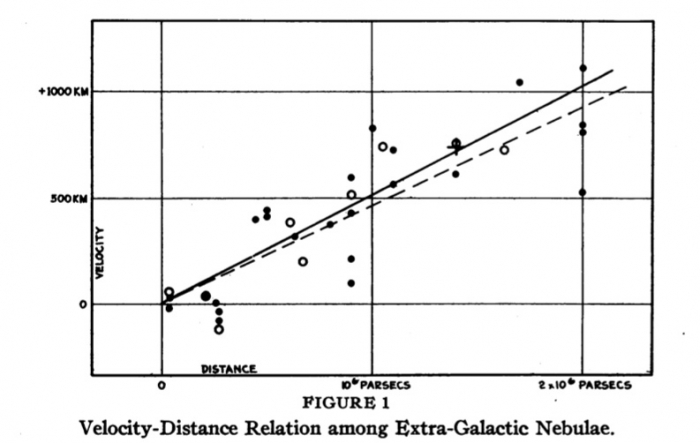
\includegraphics[width=\textwidth]{hubbleslaw}
        \caption{Hubbles Law}
        \label{fig:hubbleslaw}
\end{figure}

The observed \emph{redshifts} couldn't be explained by the proper motion of
the galaxies, instead this phenomenon was caused by the continuos expansion
of our universe.

An expanding universe was first theorized by Friedmann in 1922, before Hubble's
observations, as a consequence of the field equations of the theory of the
\emph{General Relativity} (GR). The starting point of Friedmann derivation was
an elegant and powerful assumption about the structure of our universe:
the \emph{Cosmological Principle}.

\subsection{The Cosmological Principle}\label{ss:cosmological_principle}

The matter in the universe we observe is clustered in gravitationally bound
structures, but observations at large scale (\SI{> 100}{\mega\parsec}) shows
that the place we call home appears to obey the \emph{Cosmological
Principle}:  

\begin{principle}[Cosmological Principle]
        On the largest scales, the universe is spatially homogeneous and isotropic.
\end{principle}

Note that this principle is valid for every possible observer in the
universe. We see an homogeneous and isotropic universe from our planet, and
we believe that any other observer in the universe does: there's no special
place in our universe.

There are two main piece of evidence for the cosmological principle:

\begin{itemize}
        \item The \emph{Comsmic Microwave Background Radiation} (CMB): an almost
        uniform sea of photons which fills all space and provides a snapshot of the
        universe at \num{\sim 380000} years after its birth. The CMB
        presents small fluctuations in temperature with a characteristic
        scale:

        \begin{equation}
                \frac{\var{T}}{T} \sim \num{e-5}
        \end{equation}

        \item A relevant number of \emph{redshift surveys} show that the
        distribution of stars looks increasengly smooth on larger scales.
\end{itemize}

The acceptance of such a profound statement it's the prologue to the
description of the geometry of \emph{spacetime}. 

\subsection{The FLRW Metric}\label{ss:flrw}

Friedmann, Lema\^itre, Robertson and Walker during the 1920-1930s proved
independently that the most generic metric based on the cosmological
principle is the Friedmann-Lema\^itre-Robertson-Walker (FLRW) metric:

\begin{equation}
        \dd{s}^2 = -c^2\dd{t^2} + a\qty(t)^2\qty[\dd{\chi}^2 +
        f_k\qty(\chi)^2\dd{\Omega}^2]
        \label{eq:flrw}
\end{equation}

Where:

\begin{itemize}
        \item $c$ is the speed of light in vacuum;
        \item $a\qty(t)$ is a real function of time known as \emph{scale factor};
        \item $k$ is a real number which parametrizes the spatial curvature of the
        spacetime. Due to the homogeneity and isotropy of space, $k$ is at most a
        function of time. For a fixed time $k$ is a constant and:

        \begin{itemize}
                \item $k = 0$ $\rightarrow$ flat universe;
                \item $k > 0$ $\rightarrow$ open universe;
                \item $k < 0$ $\rightarrow$ closed universe.
        \end{itemize}

        in particular:

        \begin{equation}
                f_k\qty(\chi) =
                        \begin{cases}
                                 \chi & \qif k = 0 \\
                                 \sqrt{k}^{-1} \sin(\sqrt{k} \chi) & \qif k > 0 \\
                                 \sqrt{\abs{k}}^{-1} \sinh(\sqrt{\abs{k}} \chi) & \qif k < 0
                        \end{cases}
        \end{equation}
        \item and $\dd{\Omega}^2 = \dd{\theta}^2 + \sin[2](\theta) \dd{\phi}^2$
        is the metric of the unitary sphere.
\end{itemize}

The FLRW metric in \autoref{eq:flrw} is invariant under the following transformation:

\begin{equation}
        \begin{split}
                \chi & \rightarrow \frac{\chi}{\lambda} \\
                k & \rightarrow \lambda k \\
                a & \rightarrow \lambda a
        \end{split}
\end{equation}

so it is possible to set:

\begin{align}
k & = 0,\pm 1 \\
a\qty(t_0) & = 1
\end{align}

where $t_0$ is the present time and the function $f_k$ becomes: 

        \begin{equation}
                f_k\qty(\chi) =
                        \begin{cases}
                                 \chi & \qif k = 0 \\
                                 \sin \chi & \qif k = 1 \\
                                 \sinh \chi & \qif k = -1 
                        \end{cases}
        \end{equation}

We can immediately note that the valid geometry for an homogeneous
and isotropic spacetime are either flat, spherical or hyperbolic.

\subsection{The Comoving Distance and the Hubble Parameter}

Consider two points in a slice of space in the spacetime ($t = t_*$): $p_1$,
$p_2$. The physical distance between them is calculated using the FLRW
metric for a fixed time:

\begin{equation}
        \dd{s} = a\qty(t_*)\sqrt{\dd{\chi}^2 +
        f_k^2\qty(\chi)\dd{\Omega}^2}
\end{equation}

integrating between $p_1$ and $p_2$, we obtain:

\begin{equation}
        d_{\text{phys}} = a\qty(t_*)d_{\text{co}}
        \label{eq:dd}
\end{equation}

where $d_{\text{co}}$ is the comoving distance, the distance in comoving
coordinates, which expand in the same way as space, and $d_\text{phys}$ is
the proper or physical distance.

Taking the time derivative of \autoref{eq:dd}:

\begin{equation}
        v_{\text{phys}} = \dot a\qty(t) d_{\text{co}} = \frac{\dot a\qty(t)}{a\qty(t)} d_{\text{phys}}
\end{equation}

where $v_{\text{phys}}$ is the physical or proper velocity and the function:

\begin{equation}
        H\qty(t) = \frac{\dot a\qty(t)}{a\qty(t)}
        \label{eq:hubble_parameter}
\end{equation}

is called the \emph{Hubble parameter} and its present day value $H\qty(t_0)
\equiv H_0$ is the \emph{Hubble's constant}, introduced in
\autoref{ss:hubbleslaw}. The Hubble's constant is a cosmological
parameter of our standard cosmological model and has a positive value,
indicating that we live in an expanding universe.

\subsection{The Dynamics of Spacetime}

The evolution of the scale factor $a$ introuced in \autoref{ss:flrw} is
governed by Einstein field equations of GR:

\begin{equation}
        G_{\mu \nu} = \frac{8 \pi G}{c^2} T_{\mu \nu}
        \label{eq:einstein}
\end{equation}

where:

\begin{itemize}
        \item $G_{\mu \nu}$ is the Einstein tensor, which describes the
        geometry of the spacetime;
        \item $G$ is the universal gravitational constant;
        \item $T_{\mu \nu}$ is the energy-momentum tensor, responsible for
        the energy and momentum of matter.
\end{itemize}

Einstein fields equations of GR relate the geometry of the spacetime to the
distribution of matter within it. Assuming the cosmological principle, we
can choose $T_{\mu \nu}$ to be the energy-momentum tensor of a perfect
fluid, which can be completely characterized by its density and pressure:

\begin{equation}
         T_{\mu \nu} = (\rho c^2 + P)u_\mu u_\nu + P g_{\mu \nu} 
         \label{eq:energy_momentum_tensor}
\end{equation}

Substituting \autoref{eq:flrw} and \autoref{eq:energy_momentum_tensor} in
\autoref{eq:einstein}, the field equations reduces to two equations for the
time evolution of the scale factor, known as \emph{Friedmann equations} and
written by Friedmann himself in 1922:

\begin{align}
        \qty(\frac{\dot a\qty(t)}{a\qty(t)})^2 & = \frac{8\pi G}{3} \rho\qty(t)
        - \frac{k\qty(t) c^2}{a^2\qty(t)}
        \label{eq:friedmann_1} \\
        \frac{\ddot a\qty(t)}{a\qty(t)} & = -\frac{4\pi G}{3}
        \qty(\rho\qty(t) + \frac{3 P\qty(t)}{c^2})
        \label{eq:friedmann_2}
\end{align}

The Friedmann equations constitutes a system of two differential equations
with three variables quantity: $a\qty(t)$, $\rho\qty(t)$ and $P\qty(t)$.
The last equation we need to close the system can be deduced from the
conservation of the energy-momentum tensor:

\begin{equation}
        \partial_\mu T^{\mu \nu} = 0 
\end{equation}

It's the \emph{continuity equation}, which express the conservation of energy in a
comsmological setting:

\begin{equation}
        \dot \rho + 3 H \qty(\rho + \frac{P}{c^2}) = 0
        \label{eq:continuity}
\end{equation}

A state equation of the kind $P = P\qty(\rho)$ can be specified to
integrate the continuity equation and determine how the energy density
depends on the scale factor. We guess a generic and simple shape for the
state equation of each component of the cosmological fluid:

\begin{equation}
        P = w \rho c^2 
        \label{eq:state}
\end{equation}

where $w$ is a parameter typical of each component.
Using \autoref{eq:state} in \autoref{eq:continuity} we obtain:

\begin{equation}
        \frac{\dot \rho}{\rho} = -3\qty(1 + w) \frac{\dot a}{a} 
\end{equation}

integrating over time from $t_0$ to a generic time $t$ and using the fact
that $a\qty(t_0) = 1$:

\begin{equation}
        \rho_w\qty(t) = \rho_{w,0} a^{-3\qty(1 + w)} 
\end{equation}

where $\rho_{0,w}$ is the present day energy density.
Therefore the total energy density for the cosmological fluid is:

\begin{equation}
        \rho_{\text{tot}} = \sum_w \rho_w 
\end{equation}

and \autoref{eq:friedmann_1} becomes:

\begin{equation}
        H^2\qty(t) = \frac{8\pi G}{3} \rho_{\text{tot}}\qty(t) -
        \frac{k\qty(t) c^2}{a^2\qty(t)}
\end{equation}

where we have used \autoref{eq:hubble_parameter}. The curvature parameter
$k$ can isolated in the right-hand side of the equation:

\begin{equation}
        \begin{split}
                \frac{k\qty(t) c^2}{a^2\qty(t)} & = 
                \frac{8\pi G \rho_{\text{tot}}\qty(t)}{3} - H^2\qty(t) \\
                \frac{k\qty(t) c^2}{a^2\qty(t)} & = 
                H^2\qty(t) \qty(\frac{8\pi G \rho_{\text{tot}}\qty(t)}{3H^2\qty(t)} - 1) \\
                k(t) & = \frac{H^2\qty(t) a^2\qty(t)}{c^2} \qty(\Omega\qty(t) - 1) \\
        \end{split}
        \label{eq:friedmann_curvature}
\end{equation}

In the last equation we have defined:

\begin{align}
        \rho_c\qty(t) & \equiv \frac{3H^2\qty(t)}{8\pi G} \\
        \Omega\qty(t) & \equiv \frac{\rho_{\text{tot}}\qty(t)}{\rho_c\qty(t)}
\end{align}

The function $\rho_c\qty(t)$ is known as the \emph{critical density}: it
represents the energy density time evolution for a flat universe ($k = 0$).
We note that in this case, the total energy density of the universe is
directly related to the Hubble parameter.

Evaluating \autoref{eq:friedmann_curvature} for $t = t_0$ and assuming a
time independent space curvature $k(t) = k$, yields:

\begin{equation}
        k = \frac{H^2_0}{c^2} \qty(\Omega_0 - 1) \\
\end{equation}

where:

\begin{equation}
        \Omega_0 \equiv \frac{\rho_0}{\rho_{c,0}} = \sum_w
        \frac{\rho_{w,0}}{\rho_{c,0}} \equiv \sum_w \Omega_w
\end{equation}

The adimensional quantities $\Omega_w$ are the \emph{density parameters}
for each fluid component. Note that even though we have omitted the $0$
subscript, the density parameters refer to the fraction of energy observed
today, as the definition implies.

The density parameters sum to:

\begin{equation}
        \sum_w \Omega_w = 1 + \frac{kc^2}{H^2_0} 
\end{equation}

as a consequence, if we live in a flat universe then we must have $\sum_w
\Omega_w = 1$. Any excess energy density, with $\sum_w \Omega_w > 1$ means
that we necessarily live in a positively curved universe with $k = +1$. Any
deficit in energy, with $\sum_w \Omega_w < 1$ gives rise to a negatively
curved $k = 1$ universe. Measuring the present day total energy density 
$\rho_{\text{tot},0}$ and the Hubble constant $H_0$, gives us the
opportunity to have knowledge of the spatial geometry of our universe. 

\section{The CMB Radiation}

\begin{figure}
        \centering
        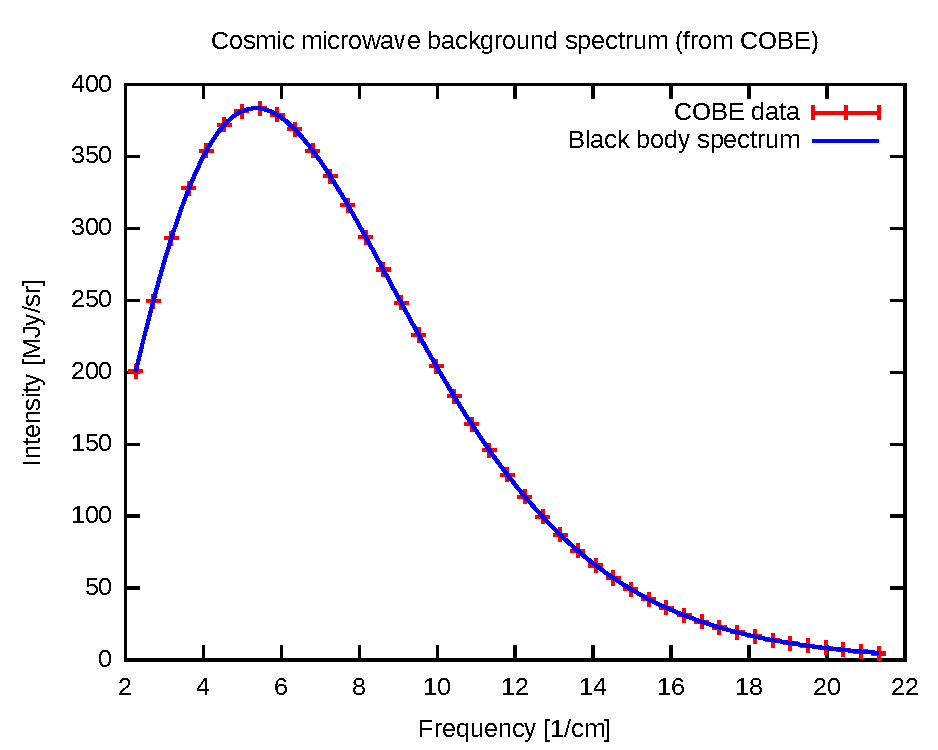
\includegraphics[width=\textwidth]{CMB_Spectrum_COBE}
        \caption{CMB Spectrum COBE}
        \label{fig:cmb_spectrum_cobe}
\end{figure}

\section{The CMB Temperature Anisotropies}

\begin{figure}
        \centering
        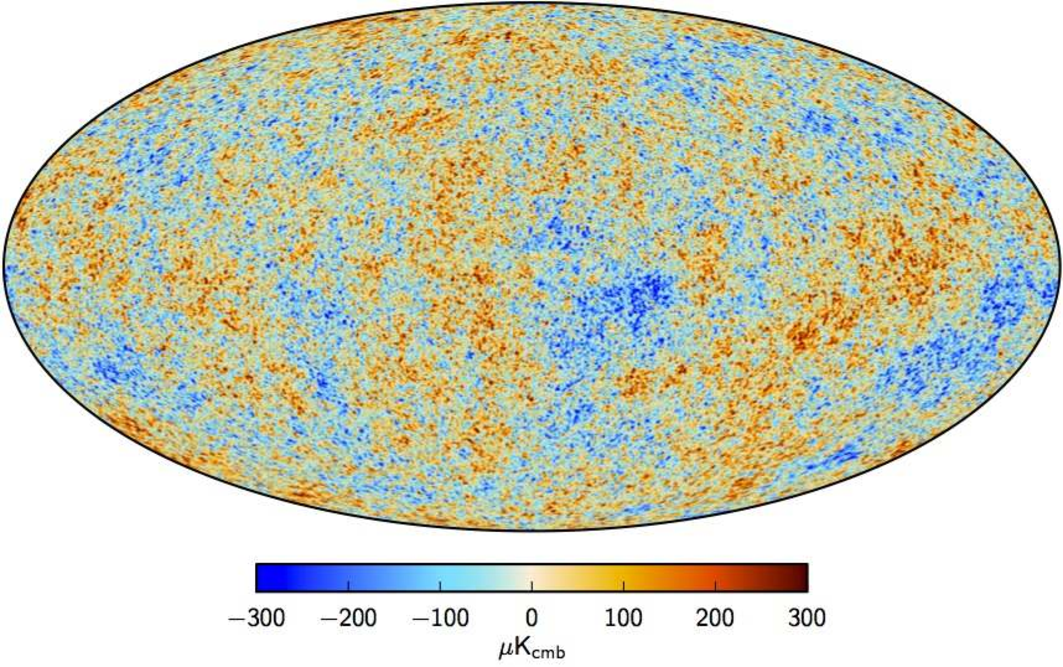
\includegraphics[width=\textwidth]{Planck_CMB}
        \caption{CMB Anisotropies Planck}
        \label{fig:plack_cmb}
\end{figure}

\section{The CMB Polarization}
